% article example for classicthesis.sty
\documentclass[11pt,a4paper]{scrartcl} % KOMA-Script article 
\usepackage{lipsum}
\usepackage{url}
\usepackage[LabelsAligned]{currvita} % nice cv style
\usepackage[nochapters]{classicthesis} % nochapters
\usepackage{tikz}
\usepackage{amsthm}
\usepackage{setspace}
\usepackage[round]{natbib}
\usetikzlibrary{calc,shapes,arrows,automata,trees,shadows,decorations.pathmorphing,positioning,
shapes.misc,shapes.arrows,chains,matrix,scopes,decorations.pathmorphing,backgrounds}
\renewcommand*{\cvheadingfont}{\LARGE\color{Maroon}}
\renewcommand*{\cvlistheadingfont}{\large}
\renewcommand*{\cvlabelfont}{\qquad}
\begin{document}
\pagecolor{Gray!05!Bittersweet!07}
%Coverletter
\begin{cv}{\spacedallcaps{Of~Peace}}
        \begin{cvlist}{\textcolor{brown}{\spacedlowsmallcaps{Jason~N~Mansfield}}}\label{PersDat}  
            \item   Regis~University
            \item   3333\\
                    Regis Boulevard Denver \\	
                    Colorado 80221-1099
            \item   mansf843@regis.edu\\				
                    \url{http://www.regis.edu/}				
        \end{cvlist}
        \begin{cvlist}{\spacedlowsmallcaps{RC~471}}\label{irgendwas}
            \item Instructed by Professor~Henri~Tshibambe\\
             \url{http://tinyurl.com/3htorkr}
        \end{cvlist}
    \end{cv}
\clearpage
\begin{center}
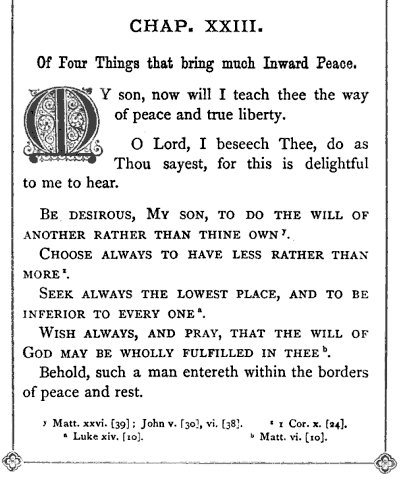
\includegraphics[scale=0.7]{ss1}
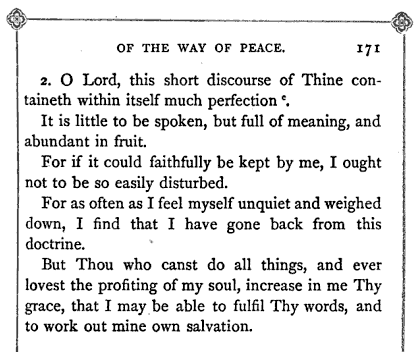
\includegraphics[scale=0.7]{ss2}
\end{center}
\clearpage

%Title
\title{\textcolor{Maroon}{\rmfamily\normalfont\spacedallcaps{Of~Peace}}}
    \author{\textcolor{brown}{\spacedlowsmallcaps{Jason N Mansfield}}}
    \date{} % no date
    
    \maketitle
    
    \begin{abstract}
  When researching various faiths is can become clear how many have the same driving factors and beliefs. The following is an overview of some writings from various religious backgrounds in which I compare them to my efforts in life. 
    \end{abstract}
       
    \tableofcontents
    \section{Judaism}
    \subsection{Abraham Isaac Kook}  
    \subsubsection{Radiant Is The World Soul}
    \begin{verse}
Full of splendor and beauty,\\
Full of life,\\
Of souls hidden,\\
Of treasures of the holy spirit,\\
Of fountains of strength,\\
Of greatness and beauty.\\
Proudly I ascend\\
Toward the heights of the world soul\\
That gives life to the universe.\\
How majestic the vision – Come, enjoy,\\
Come, find peace,\\
Embrace delight,\\
Taste and see that God is good.\\
Why spend your substance on what does not nourish\\
And your labor on what cannot satisfy?\\
Listen to me, and you will enjoy what is good,\\
And find delight in what is truly precious.\\
\end{verse} 
\textcolor{brown}{\citealp[pg. 39]{eknath}}

\subsubsection{Apply to my Journey}
The portion of Abraham Isaac Kook's poem which really strikes home to me is the mention of substance which does not nourish. This is a fact which I have found to be true over and over again. The love that God offers us is the only real nourishment. 
\subsubsection{Is it Universal}
I feel this poem is universal in the sense that it does not outline any doctrines or laws man has created to narrow down what God is.
\section{Christianity}
\subsection{Thomas A. Kempis}
\subsubsection{Four Things That Bring Much Inward Peace}
\begin{verse}
My child, now will I teach thee the way of peace and true liberty.\\
O Lord, I beseech thee, do as thou sayest, for this is delightful for me to hear.\\
Be desirous, my child, to work for the welfare of another rather than seek thine own will.\\
Choose always to have less rather than more.\\
Seek always the lowest place, and to be inferior to everyone.\\
Wish always, and pray, that the will of God may be wholly fulfilled in thee.\\
Behold, such a man entereth within the borders of peace and rest.\\
O Lord, this short discourse of thine containeth within itself much perfection. It is little to be spoken, but full of meaning, and abundant in fruit. . . . Thou who canst do all things, and ever lovest the profiting of my soul, increase in me thy grace, that I may be able to fulfill thy words, and to work out mine own salvation.
\end{verse}
\textcolor{brown}{\citealp[pg. 199]{eknath}}

\subsubsection{Apply to my Journey}
This applies specifically to me with the struggle I have with learning modesty and self control. This poem is a critical one for any military man to read. It offers a sense of peace and satisfaction that the daily struggle cannot. It sometimes is difficult to be humble especially when it can be perceived as weakness. I find most of the time it creates better leaders and skilled listeners. 
\subsubsection{Is it Universal}
Although a Christian based poem, "Four Things That Bring Inward Peace" would easily tie in with belief structures such a Buddhism, Dioism, Surfism and so forth.
    \section{Hinduism}
    \subsection{Kabir}
\subsubsection{The~Temple~Of~The~Lord}
\begin{verse}
As oil is in the oil seed, 
And fire is in the flint,
So the Lord within thee, unrevealed.
Follow thy Master's simple and true instructions,
Keep vigil strict at midnight and so find Him.\\
As fragrance is within the flower's blossom. So is the Lord within thee, unrevealed. But, the musk-deer searches for musk in forest grass. So does man search for Him outside And finds Him not. \\
As the pupil is within the eye itself, So is the Lord within thy body; But fools know not this simple fact, And search for Him elsewhere. \\
As air pervades all space, But none can see it, So does the Lord pervade the body; But He remains to each one unrevealed, Since the lodestone of the heart is not attached to Him. \\
0 man, the object of supremest value, For which you search throughout the world, is here within you, But the veil of Illusion ever separates you from Him. Tear the veil boldly asunder and you will find Him.\\ 
My Lord is living in each human being; There is no bridal bed without the Bridegroom. But blessed is the body In which He reveals Himself.\\ 
As fragrance is in the flower. So is the Lord within thee. But He reveals Himself in His beloved Saints; That is all you need to know. Go forth and meet them. 
\end{verse}
\textcolor{brown}{\citealp[pg. 40-41]{eknath}}

\subsubsection{Apply to my Journey}
I believe in a sense this poem would apply to my efforts to flush out sin and become a better temple for God. I do not believe that God lives within me but that I am his creation. I can see how God can be revealed through his saints.
\subsubsection{Is it Universal}
I believe portions of this poem are universal. I think there is some conflict with the belief that God is in each and every person. 
    \section{Buddhism}
    \subsection{Sutta Nipata} 
\subsubsection{The Island}  
\begin{verse}
For those struggling in midstream, in great fear of the flood, of growing old and of dying for all those I say, an island exists where there is no place for impediments, no place for clinging: the island of no going beyond.\\ 
I call it nirvana, the complete destruction of old age and dying.
\end{verse}
\textcolor{brown}{\citealp[pg. 200]{eknath}}

\subsubsection{Apply to my Journey}
This poem is very brief and comforting. The description of Nirvana sounds wonderful and could be applied to the belief of heaven. This could represent to me my struggle to draw closer to God who is my Nirvana. 
\subsubsection{Is it Universal}
The poem is short and vague enough that it could be applied to all religious groups.
    \section{Surfism}
    \subsection{Jal\={a}l ad-D\={i}n Muḥammad R\={u}m\={i} }
\subsubsection{A Garden Beyond Paradise}
\begin{verse}
Everything you see has its roots
    in the unseen world.
The forms may change,
    yet the essence remains the same.\\

Every wondrous sight will vanish,
every sweet word will fade.
    But do not be disheartened,
The Source they come from is eternal
growing, branching out,
    giving new life and new joy.\\

Why do you weep?
That Source is within you,
and this whole world
    is springing up from it.\\

The Source is full,
its waters are ever-flowing;
    Do not grieve,
    drink your fill!
Don't think it will ever run dry
This is the endless Ocean!\\

From the moment you came into this world,
a ladder was placed in front of you
    that you might transcend it.\\

From earth, you became plant,
from plant you became animal.
Afterwards you became a human being,
endowed with knowledge, intellect and faith.\\

Behold the body, born of dust—
    how perfect it has become!\\

Why should you fear its end?
When were you ever made less by dying?\\

When you pass beyond this human form,
no doubt you will become an angel
and soar through the heavens!\\

But don't stop there.
Even heavenly bodies grow old.\\

Pass again from the heavenly realm
    and plunge into the ocean of Consciousness.
Let the drop of water that is you
    become a hundred mighty seas.\\

But do not think that the drop alone
becomes the Ocean
    the Ocean, too, becomes the drop!\\
\end{verse}
\textcolor{brown}{\citealp[pg. 246-247]{eknath}}

\subsubsection{Apply to my Journey}
This poem is very mystical and inspiring. It makes me think of quantum physics and all the new discoveries. This poem help me realize the complexity and wonder of this universe and superposition of others. I believe this poem helps me focus on the great wisdom we have around and through us.
\subsubsection{Is it Universal}
I do believe this poem is universal as it speaks of the wisdom and intelligent life all around us. 
     \section{Native American Shamanism}
     \subsection{Great Spirit}
     \subsubsection{Prayer To The Four Directions}
\begin{verse}
 Great Spirit of Light, come to me out of the East with the power of the rising sun. Let there be light in my words, let there be light on my path that I walk. Let me remember always that you give the gift of a new day. And never let me be burdened with sorrow by not starting over again.\\

Great Spirit of Love, come to me with the power of the North. Make me courageous when the cold wind falls upon me. Give me strength and endurance for everything that is harsh, everything that hurts, everything that makes me squint. Let me move through life ready to take what comes from the north.\\

Great Life-Giving Spirit, I face the West, the direction of sundown. Let me remember everyday that the moment will come when my sun will go down. Never let me forget that I must fade into you. Give me a beautiful color, give me a great sky for setting, so that when it is my time to meet you, I can come with glory.\\

Great Spirit of Creation, send me the warm and soothing winds from the South. Comfort me and caress me when I am tired and cold. Unfold me like the gentle breezes that unfold the leaves on the trees. As you give to all the earth your warm, moving wind, give to me, so that I may grow close to you in warmth. Man did not create the web of life, he is but a strand in it. Whatever man does to the web, he does to himself. \\
\end{verse}
\textcolor{brown}{\citealp{native}}

\subsubsection{Apply to my Journey}
I really enjoy the portion of this poem where the author speaks of the web of life, "Man did not create the web of life, he is but a strand in it~\citealp{native}" This is awe inspiring. It points out that even the Native Americans believed in a creator. This poem is very beautiful and descriptive about the wonderful environment God has made for us. Much of my worship and prayer is done in the wilderness.
\subsubsection{Is it Universal}
This poem can be enjoyed and recognized by all faiths without question. The Native American really have a strong grasp of the physical world blending with the spiritual. 

  % bib stuff
\clearpage
    \nocite{*}
    \addtocontents{toc}{\protect\vspace{\beforebibskip}}
    \addcontentsline{toc}{section}{\refname}    
    \bibliographystyle{plainnat}
    \bibliography{cite}
\end{document}